%  LaTeX support: latex@mdpi.com
%  In case you need support, please attach all files that are necessary for compiling as well as the log file, and specify the details of your LaTeX setup (which operating system and LaTeX version / tools you are using).

%=================================================================
\documentclass[journal,article,atmosphere,submit,moreauthors,pdftex]{Definitions/mdpi}

% If you would like to post an early version of this manuscript as a preprint, you may use preprint as the journal and change 'submit' to 'accept'. The document class line would be, e.g., \documentclass[preprints,article,accept,moreauthors,pdftex]{mdpi}. This is especially recommended for submission to arXiv, where line numbers should be removed before posting. For preprints.org, the editorial staff will make this change immediately prior to posting.

%--------------------
% Class Options:
%--------------------
%----------
% journal
%----------
% Choose between the following MDPI journals:
% acoustics, actuators, addictions, admsci, aerospace, agriculture, agriengineering, agronomy, ai, algorithms, animals, antibiotics, antibodies, antioxidants, applmech, applsci, arts, asc, asi, atmosphere, atoms, axioms, batteries, bdcc, behavsci , beverages, bioengineering, biology, biomedicines, biomimetics, biomolecules, biosensors, brainsci , buildings, cancers, carbon , catalysts, cells, ceramics, challenges, chemengineering, chemistry, chemosensors, children, civileng, cleantechnol, climate, clockssleep, cmd, coatings, colloids, computation, computers, condensedmatter, cosmetics, cryptography, crystals, dairy, data, dentistry, designs , diagnostics, diseases, diversity, drones, econometrics, economies, education, ejbc, ejihpe, electrochem, electronics, endocrines, energies, entropy, environments, epigenomes, est, fermentation, fibers, fire, fishes, fluids, foods, forecasting, forests, fractalfract, futureinternet, futurephys, galaxies, games, gastrointestdisord, gels, genealogy, genes, geohazards, geosciences, geriatrics, hazardousmatters, healthcare, hearts, heritage, highthroughput, horticulturae, humanities, hydrology, ijerph, ijfs, ijgi, ijms, ijtpp, informatics, information, infrastructures, inorganics, insects, instruments, inventions, iot, j, jcdd, jce, jcm, jcp, jcs, jdb, jfb, jfmk, jimaging, jintelligence, jlpea, jmmp, jmse, jne, jnt, jof, joitmc, jpm, jrfm, jsan, land, languages, laws, life, literature, logistics, lubricants, machines, magnetochemistry, make, marinedrugs, materials, mathematics, mca, medicina, medicines, medsci, membranes, metabolites, metals, microarrays, micromachines, microorganisms, minerals, modelling, molbank, molecules, mps, mti, nanomaterials, ncrna, ijns, neurosci, neuroglia, nitrogen, notspecified, nutrients, oceans, ohbm, optics, particles, pathogens, pharmaceuticals, pharmaceutics, pharmacy, philosophies, photonics, physics, plants, plasma, pollutants, polymers, polysaccharides, preprints , proceedings, processes, prosthesis, proteomes, psych, publications, quantumrep, quaternary, qubs, reactions, recycling, religions, remotesensing, reprodmed, reports, resources, risks, robotics, safety, sci, scipharm, sensors, separations, sexes, signals, sinusitis, smartcities, sna, societies, socsci, soilsystems, sports, standards, stats, surfaces, surgeries, sustainability, sustainableworld, symmetry, systems, technologies, telecom, test, tourismhosp, toxics, toxins, transplantology, tropicalmed, universe, urbansci, vaccines, vehicles, vetsci, vibration, viruses, vision, water, wem, wevj

%---------
% article
%---------
% The default type of manuscript is "article", but can be replaced by:
% abstract, addendum, article, benchmark, book, bookreview, briefreport, casereport, changes, comment, commentary, communication, conceptpaper, conferenceproceedings, correction, conferencereport, expressionofconcern, extendedabstract, meetingreport, creative, datadescriptor, discussion, editorial, essay, erratum, hypothesis, interestingimages, letter, meetingreport, newbookreceived, obituary, opinion, projectreport, reply, retraction, review, perspective, protocol, shortnote, supfile, technicalnote, viewpoint
% supfile = supplementary materials

%----------
% submit
%----------
% The class option "submit" will be changed to "accept" by the Editorial Office when the paper is accepted. This will only make changes to the frontpage (e.g., the logo of the journal will get visible), the headings, and the copyright information. Also, line numbering will be removed. Journal info and pagination for accepted papers will also be assigned by the Editorial Office.

%------------------
% moreauthors
%------------------
% If there is only one author the class option oneauthor should be used. Otherwise use the class option moreauthors.

%---------
% pdftex
%---------
% The option pdftex is for use with pdfLaTeX. If eps figures are used, remove the option pdftex and use LaTeX and dvi2pdf.

%=================================================================
\firstpage{1}
\makeatletter
\setcounter{page}{\@firstpage}
\makeatother
\pubvolume{xx}
\issuenum{1}
\articlenumber{5}
\pubyear{2020}
\copyrightyear{2020}
%\externaleditor{Academic Editor: name}
\history{Received: date; Accepted: date; Published: date}
%\updates{yes} % If there is an update available, un-comment this line

%% MDPI internal command: uncomment if new journal that already uses continuous page numbers
%\continuouspages{yes}

%------------------------------------------------------------------
% The following line should be uncommented if the LaTeX file is uploaded to arXiv.org
%\pdfoutput=1

%=================================================================
% Add packages and commands here. The following packages are loaded in our class file: fontenc, inputenc, calc, indentfirst, fancyhdr, graphicx,epstopdf, lastpage, ifthen, lineno, float, amsmath, setspace, enumitem, mathpazo, booktabs, titlesec, etoolbox, tabto, xcolor, soul, multirow, microtype, tikz, totcount, amsthm, hyphenat, natbib, hyperref, footmisc, url, geometry, newfloat, caption

%=================================================================
%% Please use the following mathematics environments: Theorem, Lemma, Corollary, Proposition, Characterization, Property, Problem, Example, ExamplesandDefinitions, Hypothesis, Remark, Definition, Notation, Assumption
%% For proofs, please use the proof environment (the amsthm package is loaded by the MDPI class).

%=================================================================
% Full title of the paper (Capitalized)
\Title{Application of a Cut-Cell Immersed Boundary Method for Wildfire Simulation over Complex Terrain}

% Author Orchid ID: enter ID or remove command
\newcommand{\orcidauthorA}{0000-0000-000-000X} % Add \orcidA{} behind the author's name
%\newcommand{\orcidauthorB}{0000-0000-000-000X} % Add \orcidB{} behind the author's name

% Authors, for the paper (add full first names)
\Author{Marcos Vanella $^1$, Kevin McGrattan $^1$, Randall McDermott $^1$, Glenn Forney $^1$, William Mell $^2$, Emanuele Gissi $^3$, and Paolo Fiorucci $^4$}

% Authors, for metadata in PDF
\AuthorNames{Marcos Vanella, Kevin McGrattan, Randall McDermott, Glenn Forney, William Mell, Emanuele Gissi, and Paolo Fiorucci}

% Affiliations / Addresses (Add [1] after \address if there is only one affiliation.)
\address{%
$^{1}$ \quad National Institute of Standards and Technology, Gaithersburg, Maryland, USA \\
$^{2}$ \quad U.S. Forest Service, Seattle, Washington, USA \\
$^{3}$ \quad Corpo nazionale dei Vigili del fuoco, Savona, Italy \\
$^{4}$ \quad CIMA Research Foundation, Savona, Italy}

% Contact information of the corresponding author
\corres{Correspondence: marcos.vanella@nist.gov}


\abstract{A method for the large-eddy simulation (LES) of wildfire spread over complex terrain is presented. In this scheme, a cut-cell immersed boundary method (CC-IBM) is used to render the complex terrain, defined by a tessellation, on a rectilinear Cartesian grid. Discretization of scalar transport equations for chemical species is done via a finite volume scheme on cut-cells defined by the intersection of the terrain geometry and the Cartesian cells. Momentum transport and heat transfer close to the immersed terrain are handled using dynamic wall models and a direct forcing immersed boundary method. Further, atmospheric wind conditions are specified using a mean forcing concept. Additionally, three basic approaches have been explored to model fire spread: (1) representing the vegetation as a collection of Lagrangian particles, (2) representing the vegetation as a semi-porous boundary, and (3) representing the fire spread using a level set method in which the fire spreads as a function of terrain slope, vegetation type, and wind speed. Several test and validation cases are reported to demonstrate the capabilities of this novel wildfire simulation methodology.}

\keyword{complex terrain; fire spread; immersed boundary method; level sets}


\begin{document}


\section{Introduction}

In the past few decades, wildland and wildland-urban interface (WUI) fires have received substantial attention due to their destructive nature and extensive cost in lives and property~\cite{thomas_2017,mcdermott_2019,richards_2020}. A large body of literature can be found on the subject, as seen in various review articles~\cite{Papadopoulos_2011,Bakhshaii_2019,mcdermott_2019}. Due to the complex nature of fire, limited computing resources, and the needs of planners and first responders, most models of wildfires have historically relied on simplified field-tested rules and correlations. Among these, the rate of spread model of Rothermel~\cite{Rothermel:1972} assumes quasi-steady state surface fire conditions and takes as inputs fuel properties, wind, terrain slope, and moisture that can be measured {\em in situ}. Fuel models have been cataloged~\cite{Anderson:1982}, and their parameters defined so that model users can select and combine the most appropriate listed fuels. Rothermel's rate of spread formula is still widely used, and has been implemented in several simulation tools~\cite{Finney:FARSITE,Bova:IJWF2015,mcgratta_2013,Coen:2,Coen:2015,LAUTENBERGER_2013,Coen:2013,Mandel:2009,Mandel:2011,Mandel:2014,Kochanski:2016}, enabling a range of planning and operational forecasting capabilities.

Wildland fire modeling typically focuses on tracking the fire front, which can have a complex shape that moves and deforms based on local conditions like fuel loading, moisture content, wind, and terrain. The fire front requires a mathematical representation. The Lagrangian approach is based on a polygonal mesh of control markers that represents the front~\cite{Finney:FARSITE,Bova:IJWF2015}. On the other hand, an Eulerian representation allows for a fixed two-dimensional mesh on which the fire front is defined implicitly by a scalar field. This scalar field is called the level set function and numerical methods that solve for it in time are called Level Set Methods (LSM)~\cite{Sethian:1999,Osher:2006}. Some wildfire solvers that use LSM to track the fire front are described in references~\cite{coen_2013,Bova:IJWF2015,mcgratta_2013,LAUTENBERGER_2013}. A practical comparison of the two techniques as implemented in the Fire Dynamics Simulator (FDS)~\cite{Mell:IJWF2007} and FARSITE~\cite{Finney:FARSITE} is provided in reference~\cite{Bova:IJWF2015}.

Because the spread rate of the fire front depends in part on the local wind conditions, a well resolved wind field over complex terrain should improve the accuracy of the overall model. The de facto physics-based technique for practical simulation of wind is Large Eddy Simulation (LES)~\cite{coen_2013,Mell:IJWF2007}. For fire simulation over complex terrain, a range of techniques are being developed, in particular, in the coupling of the fire and the wind. For fast simulation of outdoor fires, an immersed boundary method has been interfaced with a Level Set scheme~\cite{Bova:IJWF2015} and the Rothermel fire spread model. The wind speed input for Rothermel's model results from the local velocity over the terrain which is affected by fire buoyancy and flow evolution. These are in turn also influenced by wind atmospheric conditions, accounted for within simulations using a mean wind forcing concept. This is a first step at implementing a level set approach in a LES wind calculation with combustion. It is recognized that, in the empirically-based development of the Rothermel formula, the wind speed was not influenced by the local buoyancy induced flow.

In the following section the mathematical model for fire spread over complex terrain is described. The description of the terrain discretization is provided in section~\ref{sec:terraindisc}. The various fire spread methods are described in section~\ref{sec:firespread}, and the atmospheric boundary conditions in section~\ref{sec:wind}. Some flat terrain simulations are compared to experimental data, and a complex terrain simulation is compared to an actual wildfire in section~\ref{sec:numexp}. 


\section{Mathematical Model} \label{sec:matmodel}

For fire modeling on the gas phase, FDS employs a low Mach approximation for thermally driven buoyant and stratified flows~\cite{Rehm:1}. Under this assumption the pressure field $p$ can be viewed as the summation of two components: a background pressure $\bar{p}(z,t)$ used on the equation of state (the ideal gas law is used), and a hydrodynamic pressure $\tilde{p}(x,y,z,t)$ resulting from fluid motion.

Consider a mixture composed of $N$ chemical species $\alpha$, moving on a fixed point $\mathbf{x}$ in space with a mass weighted average velocity $\mathbf{u}(\mathbf{x},t)$. If $\rho(\mathbf{x},t)$ is the mixture density, the mass fraction for species $\alpha$ is $Y_\alpha = \rho_\alpha / \rho$, where $\rho_\alpha(\mathbf{x},t)$ is the species mass density and $\rho = \sum \rho_\alpha$. The scalar transport and momentum equations take the form:
\begin{eqnarray}
   \frac{\partial \rho Y_\alpha}{ \partial t} + \nabla \cdot ( \rho Y_\alpha  \mathbf{u} ) &=& - \nabla \cdot \mathbf{J_{d}}_\alpha + \dot{m}_\alpha'''  +
    \dot{m}_{b,\alpha}'''\; , \; \alpha=1,\dots,N \label{eqn:spectran} \\
    \frac{\partial \mathbf{u}}{\partial t} - \mathbf{u} \times \boldsymbol{\omega} + \nabla H - \tilde{p} \, \nabla \left( 1/\rho\right) &=&
    \frac{1}{\rho} \left[ (\rho-\rho_0) \mathbf{g} + \mathbf{f}_{b} + \nabla \cdot \boldsymbol{\tau} \right] \label{eqn:momtran}
\end{eqnarray}
where $\mathbf{J_{d}}_\alpha=- \rho D_\alpha \boldsymbol{\nabla} Y_\alpha$ are the diffusive fluxes for component $\alpha$. Fick's Law for binary diffusion respect to a background species is assumed, $D_\alpha$ is the diffusivity of $\alpha$ respect to the background species.  To enforce realizability, $\sum_\alpha \mathbf{J_{d}}_\alpha = 0$, we lump errors in diffusive transport into the most abundant species locally \cite{McDermott:2015}. The volumetric combustion source term for species $\alpha$ is $\dot{m}_\alpha'''(\mathbf{x},t)$  and $\dot{m}_{b,\alpha}'''$ is the contribution to species $\alpha$ from subgrid particle gasification. In the momentum equation the head is $H=|\mathbf{u}|^2/2 + \tilde{p}/\rho$, $\tilde{p}$ is the perturbation pressure, and $\rho_0(z)$ is an equlibrium density.  The gravity vector is $\mathbf{g}=(0,0,g_z)$, $\mathbf{f}_{b}$ is the particle force term, and $\boldsymbol{\tau}$ is a tensor accounting for molecular and subgrid turbulent stresses parameterized by an effective eddy viscosity model. This last model is employed by default in large-eddy simulation (LES) of outdoor fires. Details of the model equations and their derivation are found in \cite{mcgratta_2013tr}.

Conservation of energy is achieved by forcing flow field to obey the following thermodynamic divergence constraint:
\begin{eqnarray}
    ( \nabla \cdot \mathbf{u} )^{th} &=&
    \left[ \frac{1}{\rho c_p T} - \frac{1}{\bar{p}} \right]
    \frac{\partial \bar{p}}{\partial t} + \frac{w \rho_0 g_z}{\rho c_p T} \nonumber \\
    &+& \frac{1}{\rho c_p T} \left[ \dot{q}''' + \dot{q}_b''' - \nabla \cdot \dot{\mathbf{q}}'' - \mathbf{u} \cdot \nabla (\rho h_s) \right] \nonumber \\
    &+& \frac{1}{\rho} \sum_\alpha \left( \frac{\overline{W}}{W_\alpha} - \frac{h_{s,\alpha}}{c_p T} \right) \left[ \dot{m}_\alpha'''  + \dot{m}_{b,\alpha}''' - \nabla \cdot (\mathbf{J_{d}}_\alpha) - \mathbf{u} \cdot \nabla (\rho Y_\alpha) \right] \label{eq:divth}
\end{eqnarray}
where $h_s$ is the local sensible enthalpy, $\dot{q}''', \dot{q}_b'''$ are heat release rates due to combustion and particle gasification, $\dot{\mathbf{q}}''$ is the heat flux, sum of conduction, convection and radiation, and $T$ is the local temperature. The mixture specific heat at constant pressure and molecular weight are $c_p=\sum_{\alpha =1}^N{c_{p,\alpha} Y_\alpha}$ and $\overline{W}=\left(\sum_{\alpha =1}^N{Y_\alpha /W_\alpha} \right)^{-1}$ respectively, built from the individual species counterparts as defined. Finally, $w,\rho_0,g_z$ on the stratification term are respectively, the local vertical velocity, density for standard conditions (depends on vertical coordinate), and vertical gravity acceleration. This thermodynamic divergence is derived from and acts as a proxy for the sensible enthalpy evolution equation~\cite{mcdermo_2014}. Equation (\ref{eq:divth}) is derived by factoring the divergence from the sensible enthalpy equation and applying the ideal gas law.  Given a background pressure and a local mass density the local temperature is computed from the ideal gas law as $T = \bar{p} \overline{W} / (\rho R) $.


\section{Terrain description and discretization} \label{sec:terraindisc}

In figure~\ref{Fig:figure_1}a, a terrain is represented by its surface triangulation within an FDS cartesian mesh. Some cartesian cells and faces belonging to this mesh are transversed by the terrain surface. The remainder polyhedra and polygons that lay on the gas side of this intersected cartesian entities are called cut-cells and cut-faces. They discretize the fluid domain in the region surrounding the solid terrain. A detail of this unstructured mesh is shown in figure~\ref{Fig:figure_1}b. The resulting cut-cells and cut-faces are of varied sizes and shapes, and situations where more than one cut-cell per cartesian cell are not uncommon. As described later, small cells pose a temporal stability constraint in explicit time integration schemes that needs to be addressed.
It is noted that a two level of refinement grid hierarchy emerges. The coarse level is defined by the Cartesian entities, whereas the fine level is defined by the cut-cell or unstructured counterparts. Methods that solve discrete model equations on these grids are called cut-cell or embedded boundary methods~\cite{berger_2016}. Reliably defining the cut-cell mesh geometric properties and topology is a complex problem on itself, omitted here in order to keep the discussion succinct.
\begin{figure}[ht]
   \centering
   \includegraphics[trim = 12mm 42mm 8mm 25mm, clip,width=1\linewidth]{./figures/SketchFig1.pdf}
   \put(-305,-5){(a)}
   \put(-95,-4){(b)}
   \caption{Sketch of regular Cartesian and cut-cell grids around terrain: (a) An unstructured cut-cell region is defined on the gas phase side around a terrain $\mathbf{T}$. (b) Detail showing a slice representative of cut-cells and regular gas cells, terrain triangulation and two refinement level interpretation.}
   \label{Fig:figure_1}
\end{figure}


\subsection{Scalar transport and energy discretization in unstructured region}

The equations for chemical species transport are discretized using the finite volume method (FV)~\cite{eymard_2000,leveque_2002}. See figure~\ref{Fig:figure_2}a. Integrating equation~\eqref{eqn:spectran} over a cut-cell $ii$ with control volume $\Omega_{ii}$:
\begin{equation}
 \int_{\Omega_{ii}} {\frac{\partial \rho Y_\alpha}{\partial t}} d \Omega + \int_{\Omega_{ii}} { \boldsymbol{\nabla} \cdot  \left(  \rho Y_\alpha \mathbf{u} \right)
      } d \Omega  = -\int_{\Omega_{ii}} { \boldsymbol{\nabla} \cdot \left(  \mathbf{J_{d}}_\alpha  \right)  } d \Omega + \int_{\Omega_{ii}} {( \dot{m}_\alpha'''+\dot{m}_{b,\alpha}''') } d \Omega \label{eq:intconvdiff}
\end{equation}
For a control volume that does not change with time, the time derivative and source terms are approximated by
\begin{eqnarray}
  \int_{\Omega_{ii}} {\frac{\partial \rho Y_\alpha}{\partial t}} d \Omega & = & \frac{\partial}{\partial t} \int_{\Omega_{ii}} {\rho Y_\alpha} d \Omega
  = \frac{\partial \widetilde{\rho \: Y_\alpha }_{ii}}{\partial t} V_{ii} \\
  \int_{\Omega_{ii}} {( \dot{m}_\alpha''' +\dot{m}_{b,\alpha}''')} d \Omega & = & (\widetilde{ \dot{m}_\alpha''' }_{ii}+ \widetilde{\dot{m}_{b,\alpha}'''}_{ii}) V_{ii} \label{eq:intcons}
\end{eqnarray}
where $V_{ii}$ is the volume of cell $ii$ and tildes imply cell averages. In the following the notation is simplified by dropping tildes, observing that quantities are cell or face averaged. Consider the FV discretization of the diffusive term (eqn.~\eqref{eq:intconvdiff}) on cut-cell $ii$ of figure~\ref{Fig:figure_2}a:
\begin{equation}
\int_{\Omega_{ii}} { \boldsymbol{\nabla} \cdot \left(  \mathbf{J_{d}}_\alpha  \right)  } d \Omega =
    \int_{\partial \Omega_{ii}} { \left( - \rho D_\alpha \boldsymbol{\nabla} Y_\alpha \right) \cdot \hat{\mathbf{n}}_{ii} } \: d \partial \Omega = \sum^{nf_c}_{k=1}
    \left( - \rho D_\alpha \boldsymbol{\nabla} Y_\alpha \right)_k \cdot \hat{\mathbf{n}}_{ii,k} \: A_k \label{eq:discfvdiffcc}
\end{equation}
The integral over the cut-cell volume has been transformed in an area integral on its $nf_c=5$ faces using the divergence theorem. As these $k$ faces with areas $A_k$ and normals out of the control volume $\hat{\mathbf{n}}_{ii,k}$ are planar by construction, the method for evaluation of their mean diffusive fluxes $\left( - \rho D_\alpha \boldsymbol{\nabla} Y_\alpha \right)_k$ will define the spatial accuracy of the discretization. A centroid to centroid (i.e. $\Delta x_{cc}$ in figure~\ref{Fig:figure_2}a) finite differences and linear interpolation are used to approximate $\boldsymbol{\nabla} Y_\alpha$ and $\rho D_\alpha$ for each face belonging to the gas phase. Also, a normal probe approach~\cite{balaras_2004} is employed to sample information from the fluid to define fluxes in boundary cut-faces.
\begin{figure}[ht]
   \centering
   \includegraphics[trim = 30mm 42mm 35mm 45mm, clip,width=1\linewidth]{./figures/SketchFig2.pdf}
   \put(-335,-5){(a)}
   \put(-95,-4){(b)}
   \caption{Sketch of cut-cell and faces: (a) Cut-cell $ii$ surrounded by gas phase regular and cut-faces (3-5), and boundary cut-faces (1-2).  (b) Interpolation sketch for wall modeled immersed boundary reconstruction of cut-face velocities.}
   \label{Fig:figure_2}
\end{figure}
Similarly, the discretization of the advective term is:
\begin{equation}
    \int_{\Omega_{ii}} { \boldsymbol{\nabla} \cdot  \left(  \rho Y_\alpha \mathbf{u} \right)} d \Omega =
     \int_{\partial \Omega_{ii}} { \left( \rho Y_\alpha \mathbf{u} \right) \cdot \hat{\mathbf{n}}_{ii} } \: d \partial \Omega =
     \sum^{nf_c}_{k=1} \left( \rho Y_\alpha \mathbf{u} \right)_k \cdot \hat{\mathbf{n}}_{ii,k} \: A_k \label{eq:discfvadvcc}
\end{equation}
where the advective flux for face $k$ is $\left( \rho Y_\alpha \mathbf{u} \right)_k = \overline{[\rho Y_\alpha]}_k \mathbf{u}_k$, and the over bar in $\overline{[\rho Y_\alpha]}_k$ means it is a flux limited interpolation to the cut-face~\cite{mcgratta_2013}. In the cut-cell region we use Godunov interpolation for the advective term. As the time integration scheme in FDS is an explicit Runge-Kutta (RK2) method, all variables in the right hand side of equations~\eqref{eq:discfvdiffcc}-\eqref{eq:discfvadvcc} are assumed known. The FV counterpart of the thermodynamic divergence expression for cut-cell $ii$ is:
\begin{eqnarray}
    ( \nabla \cdot \mathbf{u} )_{ii}^{th} \; V_{ii} &=&
    \left[ \frac{1}{(\rho c_p T)_{ii}} - \frac{1}{\bar{p}_{ii}} \right]
    \frac{\partial \bar{p}_{ii}}{\partial t} \; V_{ii} +
    \frac{w_{ii} \: \rho_0 g_z}{(\rho c_p T)_{ii}} V_{ii} \nonumber \\
    &+& \frac{1}{(\rho c_p T)_{ii}} \left[ (\dot{q}'''+ \dot{q}_b''')_{ii} V_{ii} -
    \sum_{k=1}^{nf_c} \dot{\mathbf{q}}''_{ii,k} \cdot \hat{\mathbf{n}}_{ii,k} \: A_k
    - \overline{\mathbf{u} \cdot \nabla (\rho h_s)} V_{ii} \right]  \\
    &+& \frac{1}{\rho_{ii}} \sum_\alpha \left( \frac{\overline{W}}{W_\alpha} - \frac{h_{s,\alpha}}{c_p T} \right)_{ii} \left[ (\dot{m}_\alpha'''+\dot{m}_{b,\alpha}''')_{ii} V_{ii} -
    \sum_{k=1}^{nf_c} \mathbf{J}_{\alpha,ii,k} \cdot \hat{\mathbf{n}}_{ii,k} \: A_k
    - \overline{\mathbf{u} \cdot \nabla (\rho Y_\alpha)} V_{ii} \right] \nonumber \label{eq:divth2}
\end{eqnarray}
where the over line terms refer to flux limited interpolation of corresponding scalars and terms defined with subscript $ii$ refer to cell defined quantities. All heat and mass fluxes and scalars are assumed known. Also, the vertical velocity $w_{ii}$ is interpolated to the cut-cell centroid. Details of the FDS time integration scheme can be found in references~\cite{mcgratta_2013,mcdermo_2014}. For each RK2 substep, the species transport equations are advanced in all FDS cartesian cells, and then the solution (explicit fluxes and scalar densities) recomputed on the unstructured cut-cell region. A similar procedure is done for the thermodynamic divergence.
% Small cell linking for explicit time integration.
As an explicit time integrator is used, in general there will arise cut-cells whose small-size will penalize severely the time step. For these we link their unknown number to larger surrounding cells, which in turn defines mathematically an evolution equation for the union of both linked cells. Cell linking in the context of momentum equations can be found in reference~\cite{kirk_2003}.
In FDS, the momentum equations and pressure Poisson equation are solved in the cartesian mesh. Therefore, an immersed boundary method is used to reconstruct velocities in the cut-cell region. A divergence integral equivalence argument is used to transfer the the divergence from cut-cells to under laying cartesian cells, and build the source of the Poisson equation for the pressure.


\subsection{Immersed boundary method on cut-cell region and wall modeling}

Collecting advective, shear stress and force terms in $\mathbf{F}(\mathbf{u},\mathbf{x},t)$ within equation~\ref{eqn:momtran}, the model momentum transport problem can be casted as~\cite{mcgratta_2013}:
%
\begin{eqnarray}
  \frac{\partial \mathbf{u}(\mathbf{x},t)}{\partial t} &=& - \left[ \mathbf{F}(\mathbf{u},\mathbf{x},t) + \boldsymbol{\nabla} H(\mathbf{x},t) \right ]\label{eq:LowMachMom} \\
         \nabla \cdot \mathbf{u} (\mathbf{x},t) & = & \left(\nabla \cdot \mathbf{u} \right)^{th} \label{eq:LowMachDiv}
\end{eqnarray}
%
where equation~\eqref{eq:LowMachMom} is the momentum equation, subject to a specified divergence field, provided by equation~\eqref{eq:divth}.
Boundary conditions are prescribed for $\mathbf{u}(\mathbf{x},t)$ on boundaries, including the immersed terrain.
%Classical fractional step methods for time integration of incompressible or low Mach flow are based on two operations: First, momentum transport to obtain intermediate velocities, and second, projection of velocities into a target divergence space.
The previous equations are advanced in time using a fractional step method. As illustration, consider their Forward Euler (FE) update from $t_n$ to $t_{n+1}=t_n + \Delta t$. Given $ \mathbf{u}^n=\mathbf{u}(\mathbf{x},t_n)$, $\nabla \cdot \mathbf{u}^{n+1} = \left( \nabla \cdot \mathbf{u}^{n+1} \right)^{th}$ known
%
\begin{eqnarray}
  \frac{\mathbf{u}^{n+1}-\mathbf{u}^{n}}{\Delta t} &=& - \left[ \mathbf{F}^n +  \boldsymbol{\nabla} H^n \right] \label{eq:LowMachMomEu}\\
  \nabla \cdot \mathbf{u}^{n+1} &=& \left( \nabla \cdot \mathbf{u}^{n+1} \right)^{th} \label{eq:LowMachDivEu}
\end{eqnarray}
%
where $\mathbf{u}^{n+1}$ represents a numerical solution at time $t_{n+1}$. This discrete FE update corresponds to the first sub-step of the FDS explicit RK2 integrator. As the potential field $H(\mathbf{x},t)$ does not have a time evolution equation, it is assumed responsible of enforcing the divergence condition and used on the projection step. Taking the divergence of equation~\eqref{eq:LowMachMomEu} and considering  the constraint~\eqref{eq:LowMachDivEu}, the two steps of the method are
%
\begin{enumerate}
  \item Solve Poisson equation for $H^n$:

\begin{equation}
   \nabla \cdot \boldsymbol{\nabla} H^n = - \left[ \frac{\left( \nabla \cdot \mathbf{u}^{n+1} \right)^{th} - \nabla \cdot \mathbf{u}^{n}}{\Delta t} \right] - \nabla \cdot \mathbf{F}^n \label{it:FSPoisson}
\end{equation}

  \item Obtain final velocity for step:

  \begin{equation}
     \mathbf{u}^{n+1} = \mathbf{u}^{n} - \Delta t \left[ \mathbf{F}^n +  \boldsymbol{\nabla} H^n \right] \label{it:FSProject}
   \end{equation}

   %The term $\hat{\mathbf{u}}^{n+1}=\mathbf{u}^{n} - \Delta t \mathbf{F}^n$ is known as intermediate velocity, and is a non divergence matching approximation to $\mathbf{u}^{n+1}$ (i.e. $\nabla \cdot \hat{\mathbf{u}}^{n+1} \neq \left( \nabla \cdot \mathbf{u}^{n+1} \right)^{th}$).
\end{enumerate}
%
A consequence of the projection scheme is that boundary conditions are required on the Poisson equation of step~\eqref{it:FSPoisson}. For explicit methods and stationary \textit{solid} boundaries, the corresponding boundary condition is \textit{homogeneous} Neumann for $H^n$ in $\partial \Omega,\partial \Omega_1,...,\partial \Omega_{nbods}$~\cite{perot_1993}.
Next, an approximation to the no-slip boundary condition at the immersed terrain surface is needed. To this end, a direct forcing immersed boundary method (IBM) for the momentum equations~\cite{fadlun_2000} is employed. A force field is computed on the discrete momentum equations on grid faces crossed by the immersed surfaces to approximate the no-slip boundary condition on these. In LES, the surrounding velocity field is modeled using an equilibrium boundary layer solution.

In figure~\ref{Fig:figure_2}b the velocity update in each of the gas phase cut-face centroids $d$ is done individualizing the point $B$ on the boundary and normal direction through these. Also, and external point $e_x$ through the normal $\mathbf{\hat{n}}$ is defined at a distance $\delta_{ex}$, of the order of the cartesian cells size. Known velocities and fluid parameters are interpolated from the surrounding fluid points $e_1,\dots,e_4$ to $e_x$.
This information is used to estimate a target velocity at step $n+1$, $\mathbf{\hat{u}}_d^{n+1,k-1}$ at point $d$, assuming the log law equilibrium boundary layer solution~\cite{mcgratta_2013}. The target velocity $\hat{u}_d^{n+1,k-1}$ component on the cut-face centroid is flux matched to the under-laying cartesian face $E$ velocity component $\hat{u}_E^{n+1,k-1}$. Finally, an immersed boundary force
%
\begin{equation}
F_E^k=-\frac{\hat{u}_E^{n+1,k-1}-u_E^{n}}{\Delta t} - \frac{\partial H^{n,k-1}}{\partial x}
\label{eq:FIBM}
\end{equation}
%
can be computed and used in equation~\eqref{it:FSPoisson} to take into account the presence of the body. The index $k$ refers in this context to the subiteration that can be performed in the IB force~\eqref{eq:FIBM} and projection~\eqref{it:FSPoisson}-\eqref{it:FSProject} to match final velocities with the wall modeled targets. This velocity reconstruction procedure has been combined with the level set method for fire spread described in next section.


\section{Wildland Fire Spread} \label{sec:firespread}

There are various ways of simulating wildland fire spread depending on the resolution of the underlying numerical grid. 
\begin{enumerate}
\item {\bf Particle Model:} The vegetation is represented by a collection of Lagrangian particles that are heated via convection and radiation. This model is appropriate for grid resolution of the order of 1~m or less.
\item {\bf Boundary Fuel Model:} Ground vegetation is modeled like a porous solid with a thickness equal to the height of the vegetation. This model is appropriate for grid resolution of the order of 1~m to 10~m.
\item {\bf Level Set Method:} The fire front propagates using purely empirical rules. This model is appropriate for grid resolution of the order of roughly 10~m and greater. 
\end{enumerate}
The Particle Method and Boundary Fuel Model require thermo-physical properties of the vegetative fuels and the fire spread rate is {\em predicted} by the model. The Level Set Method relies on a set of predetermined spread rates for different types of vegetation and wind speeds.

\subsection{Particle Model}

Lagrangian particles can be used to represent different types of vegetation, like leaves, grass, and so on. In the model, each type of vegetation is represented by a single particle in each computational grid cell. Most often the particle is assumed to be cylindrical in shape. The particle is assigned a diameter based on the measured surface area to volume ratio, $\sigma$. The length is relatively unimportant so long as it is assumed to be much greater than the diameter. Material properties are assigned for the wet vegetation which is assumed to dry, decompose to char, and then exothermally oxidize when exposed to heat from an oncoming fire. The drag force exerted by the collection of particles is given by:
\begin{equation}
   \mathbf{f}_{\rm b} = \frac{\rho}{2} \, C_{\rm d} \, C_{\rm s} \, \beta \, \sigma \, \mathbf{u} \, \|\mathbf{u}\|
   \label{drag}
\end{equation}
where $\rho$ is the air density, $C_{\rm d}$ is the drag coefficient, $C_{\rm s}$ is the shape factor (ratio of projected area to surface area), $\beta$ is the packing ratio, $\sigma$ is the surface area to volume ratio, and $\mathbf{u}$ is the air velocity. The diameter is specified via the surface area to volume ratio, $\sigma=2/r$ for a cylinder. The packing ratio is the volume of solid needles divided by the volume they occupy, typically denoted $\beta$. It is calculated by dividing the dry mass of vegetation per unit volume, the so-called ``bulk density,'' by the density of the dry vegetation, $\rho_{\rm d}$.

A coniferous tree (e.g. pine, spruce, fir) can be represented in FDS as a collection of Lagrangian particles forming a large cone. The trunk and heavier branches are typically neglected.


\subsection{Boundary Fuel Model}

In many simulations of wildland fire, the ground vegetation layer is too shallow to be resolved explicitly, as is done when using Lagrangian particles to represent the vegetation. In such cases, the ground vegetation can be modeled as a porous boundary consisting of a layer of dry vegetation, moisture, and air, underneath of which is hard ground~\cite{Perez-Ramirez:FT2017}. The drag exerted by the vegetation is modeled using a special velocity boundary condition, and convective heat transfer is modeled via a source term in the one-dimensional heat conduction equation that is solved through the layer of vegetation and solid ground. Thermal radiation penetrates the vegetation layer via a 1-D radiative transport equation that is used for semi-transparent solids.

The Boundary Fuel and Particle Models share the same basic input parameters and pyrolyis model. The drag exerted on the wind flowing through the vegetation is imposed as a force term in the gas phase grid cell adjacent to the boundary:
\begin{equation}
    \mathbf{f}_{\rm b} = \frac{\rho}{2} \, C_{\rm d} \, C_{\rm s} \, \beta \, \sigma \, \frac{h_{\rm b}}{\delta z} \, \mathbf{u} \, ||\mathbf{u}||
\end{equation}
where the parameters are the same as in Eq.~(\ref{drag}) except for the additional depth of vegetation, $h_{\rm b}$, height of a grid cell, $\delta z$, and $\mathbf{u}$ is the gas velocity in the first grid cell.

Thermal radiation is absorbed in depth according to a 1-D radiative transport solver. The absorption coefficient is given by:
\begin{equation}
   \kappa = C_{\rm s} \, \sigma \, \beta
\end{equation}
Thermal convection is not imposed at the interface between the gas phase and the vegetation layer, but rather is imposed via a source term in the 1-D heat conduction solver:
\begin{equation}
   \langle \dot{q}_{\rm c,b}''' \rangle = \sigma \, \beta \, \dot{q}_{\rm c}'' \quad ; \quad \dot{q}_{\rm c}'' = h \, (T_{\rm g} - T_{\rm s}) \quad \hbox{W/m}^2 \quad ; \quad  h = \frac{k}{L} \, {\rm Nu}
\end{equation}
where $\dot{q}_{\rm c}''$ the convective heat transferred to a small, cylindrical solid under the assumption that the subgrid-scale vegetation is cylindrical and the gas velocity and temperature are taken from the first gas phase grid cell adjacent to the boundary.


\subsection{Level Set Model}

For simulations of wildland fires spanning large areas that cannot be gridded finely enough to predict fire spread using a physics-based model, fire spread via level sets is an option~\cite{Bova:IJWF2015}. This approach makes use of the Rothermel-Albini~\cite{Rothermel:1972,Albini:1976} surface fire spread rate formulae and the assumption that a surface fire spreading from a point under certain wind, slope and vegetation conditions does so with an ellipse-shaped fire front with, for a given wind speed, a fixed length-to-breadth ratio~\cite{Richards:1990}. The location of a fire front is defined implicitly via a two dimensional level set scalar function $\phi(x,y,t)=0$. The advection equation for the level set function is
\begin{equation}
   \frac{D \phi(x,y,t)}{D t} =  \frac{\partial \phi}{\partial t} + \mathbf{R}_{uv} \cdot \nabla (\phi) = 0 \label{eqn:lset}
\end{equation}
where $\mathbf{R}_{uv}=(R_u,R_v)$ is the spread rate vector. The magnitude of the vector is
\begin{equation}
  \|\mathbf{R}_{uv}\|=R_0 \left(1 + \sqrt{(\boldsymbol{\phi}_W+\boldsymbol{\phi}_S) \cdot (\boldsymbol{\phi}_W+\boldsymbol{\phi}_S) } \right)
\end{equation}
where $R_0$ is the zero velocity, zero slope rate of spread that depends on the fuel properties. The vectors $\boldsymbol{\phi}_W,\boldsymbol{\phi}_S \ge 0$ are computed using the local wind and slope through empirical rules~\cite{Wilson:1980}. See Appendix 1 of reference~\cite{Bova:IJWF2015} for details on these calculations. In FDS, the level set spread model can be applied in various ways:
\begin{enumerate}
\item Only the level set simulation is performed. The wind is not affected by the terrain, and there is no fire.
\item The wind field is established over the terrain, but it is ``frozen'' when the fire ignites.
\item The wind field follows the terrain, but there is no actual fire in the simulation. It is just front-tracking.
\item The wind and fire are fully-coupled. When the fire front arrives at a given surface cell, it burns for a finite duration and with a heat release per unit area provided as part of the fuel model.
\end{enumerate}
When fully coupled to the CFD model, the level set function acts as an igniter as it reaches a new surface cell. The cell burns for a pre-determined amount of time. For cases where the depth of the fireline is less than the size of a grid cell, the burning time is extended while the burning rate is decreased so as to maintain conservation of fuel mass.



\section{Defining atmospheric wind : The Mean Forcing Concept} \label{sec:wind}

The process of steering the solution of the mass, momentum, and energy equations to match wind speed and direction gathered at random weather stations is known as \emph{data assimilation}~\cite{Kalnay:2003}. FDS uses a relatively simple data assimilation technique, a method known as \emph{nudging}, where you add a forcing term to the momentum equation to ``nudge'' the flow in the direction of the specified wind. FDS automatically drives the mean velocity components toward the desired values by adding a forcing term to the momentum equation. For example, the $u$ component equation is modified as follows:
\begin{equation}
   \frac{\partial u}{\partial t} + \ldots = \frac{u_0(z,t)-\overline{u}(z,t)}{\tau} \label{mean_forcing_u}
\end{equation}
Here, $u(\mathbf{x},t)$ is the computed velocity component, $u_0$ is the specified wind field component that can vary with height and time, and $\overline{u}$ is the average of the computed velocity component at the height $z$. The relaxation time scale, $\tau$, is an important parameter. The shorter this time scale, the faster the flow field will ``catch up'' to the mean wind, but at the expense of possibly washing out important flow structures.


\section{Numerical Experiments} \label{sec:numexp}


\subsection{Flat Terrain Fire Spread}  \label{sec:simexp}

In July and August of 1986, the Commonwealth Scientific and Industrial Research Organisation (CSIRO) of Australia conducted controlled grassland fire experiments near Darwin, Northern Territory~\cite{Cheney:IJWF1993}. July and August are in the middle of the dry season when the grasses are fully cured (dried) and the weather is warm and dry. The experiments were conducted on flat plots measuring 100~m by 100~m, 200~m by 200~m, or 200~m by 300~m. Two cases have been simulated. Case~C064 was conducted on a 100~m by 100~m plot of kerosene grass ({\it Eriachne burkittii}); Case~F19 was conducted on a 200~m by 200~m plot of kangaroo grass ({\it Themeda australis}).

Two of these experiments were originally simulated with FDS by Mell~et~al.~\cite{Mell:IJWF2007}. These simulations modeled the grass as a collection of cylindrical Lagrangian particles. Now these two experiments are also simulated using the Boundary Fuel Model (BFM)~\cite{Perez-Ramirez:FT2017} and the Rothermel-Albini fire spread algorithm~\cite{Rothermel:1972,Albini:1976}. For the experiment labelled Case~C064, fuel index 1 (Short Grass) is used, with a modified moisture fraction of 0.063. For F19, fuel index 3 (Tall Grass) is used, with a modified moisture fraction of 0.058.

Measured properties for the specific types of grasses burned in the two experiments are listed in Table~\ref{Properties_Grasses}. Properties that were not measured are listed in Table~\ref{Assumed_Properties_Grasses}. These assumed properties are typically for wood or cellulosic fuels. The moisture is modeled as water. The grass is assumed to be composed primarily of cellulose.

\begin{figure}[ht]
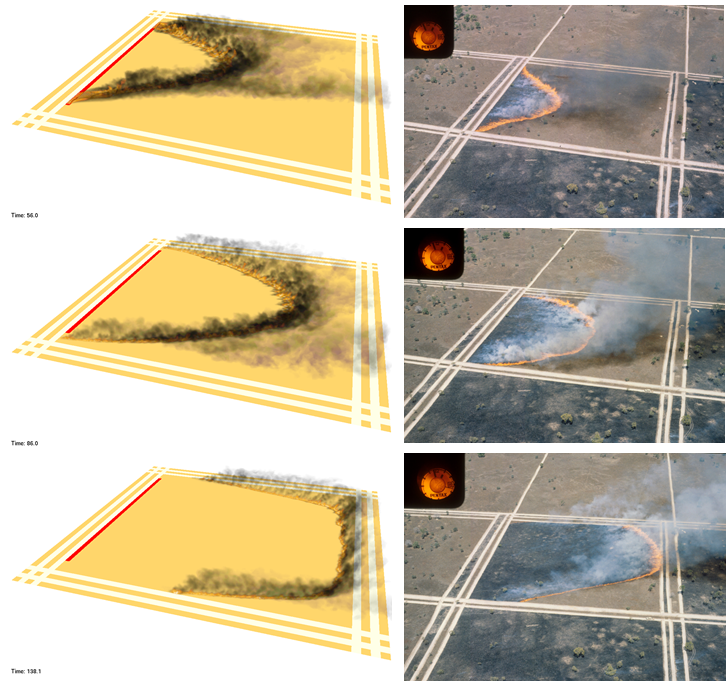
\includegraphics[width=\textwidth]{figures/F19_collage.png}
\caption{Photographs of the experiment and snapshots of the simulation of CSIRO Grassland Fire F19, 56~s, 86~s, and 138~s following ignition.}
\label{F19}
\end{figure}

Snapshots of the Lagrangian particle simulation of Case~F19 compared to photographs of the experiment are shown in Fig.~\ref{F19}. The plot of grass is 200~m by 200~m and the computational domain is 240~m by 240~m by 20~m high. The grid cells are 0.5~m cubes. The domain is subdivided into 36 individual meshes and run in parallel. A blade of grass is represented by a single cylindrically-shaped particle within a grid cell. The radius of the cylinder is derived from the measured surface area to volume ratio of the grass. Each simulated blade of grass represents many more actual blades of grass. The weighting factor is determined from the measured bulk mass per unit area. The fires in the experiments were ignited by two men carrying drip torches walking in opposite directions along the upwind boundary of the plot (the red strip in Fig.~\ref{F19}). In FDS, this action was modeled using a specified spread rate along the strip.

\begin{table}[ht]
\begin{center}
\caption[Measured properties for the CSIRO Grassland Fire cases]{Measured properties for the CSIRO Grassland Fire cases~\cite{Cheney:IJWF1993}.}
\label{Properties_Grasses}
\begin{tabular}{|l|c|c|c|}
\hline
Property                        & Units         & Case F19      & Case C064     \\ \hline \hline
Wind Speed                      & m/s           & 4.8           & 4.6           \\ \hline
Ambient Temperature             & $^\circ$C     & 34            & 32            \\ \hline
Surface Area to Volume Ratio    & m$^{-1}$      & 12240         & 9770          \\ \hline
Grass Height                    & m             & 0.51          & 0.21          \\ \hline
Bulk Mass per Unit Area         & kg/m$^2$      & 0.313         & 0.283         \\ \hline
Moisture Fraction               & \%            & 5.8           & 6.3           \\ \hline
Measured ROS                    & m/s           & 1.5           & 1.1           \\ \hline
Calculated ROS, Particle Method & m/s           & 1.5           & 1.0           \\ \hline
Calculated ROS, Boundary Fuel Method & m/s      & 3.7           & 2.5           \\ \hline
Calculated ROS, Level Set Method & m/s          & 1.3           & 0.7           \\ \hline
\end{tabular}
\end{center}
\end{table}

The predicted rates of spread for the two cases are listed in Table~\ref{Properties_Grasses}. For these simulations, the particle method is the most accurate, and the boundary fuel method over-predicts by about a factor of two. The level set method under-predicts the rate of spread, but only because of the somewhat arbitrary choice of fuel type. For a simple flat terrain scenario like this, the choice of fuel model to accompany the level set calculation largely determines the spread rate. The original FDS simulations of this experiment ~\cite{Mell:IJWF2007} also used a boundary fuel approach, with better results, work is underway to reconcile the differences. It is not surprising that the particle method does well in this scenario because it is closest to the actual physics. However, for larger domains, the boundary fuel and level set methods are better able to approximate the fire spread while the particle method would require an excessive amount of computer resources.

\begin{table}[ht]
\begin{center}
\caption[Assumed properties for dry grass and soil]{Assumed properties for various types of dried grass and soil. Note that the Pyrolysis Temperature is taken to be the temperature at which the mass loss rate peaks in the TGA experiments of Morvan and Dupuy~\cite{Morvan:CF2004}.}
\label{Assumed_Properties_Grasses}
\begin{tabular}{|l|c|c|c|}
\hline
Property                        & Units                 & Value                     & Reference                             \\ \hline \hline
Chemical Composition            & --                    & C$_6$H$_{10}$O$_5$        & Assumption                            \\ \hline
Heat of Combustion              & kJ/kg                 & 15600                     & \cite{Susott:FS1982}                  \\ \hline
Soot Yield                      & kg/kg                 & 0.015                     & \cite{SFPE:Tewarson}                  \\ \hline
Char Yield                      & kg/kg                 & 0.2                       & \cite{Susott:FS1982}                  \\ \hline
Specific Heat                   & kJ/(kg$\cdot$K)       & 1.5                       & Various sources                       \\ \hline
Conductivity                    & W/(m$\cdot$K)         & 0.1                       & Assumption                            \\ \hline
Density                         & kg/m$^3$              & 512                       & \cite{Rothermel:1972}                 \\ \hline
Heat of Pyrolysis               & kJ/kg                 & 418                       & \cite{Morvan:CF2004}                  \\ \hline
Pyrolyis Temperature            & $^\circ$C             & 200                       & \cite{Morvan:CF2004}                  \\ \hline \hline
Obukhov Length                  & m                     & -500                      & Assumption                            \\ \hline
Aerodynamic Roughness Length    & m                     & 0.03                      & Assumption                            \\ \hline
Drag Coefficient                & --                    & 2.8                       & \cite{Falkenstein-Smith:2018}         \\ \hline \hline
Soil Specific Heat              & kJ/(kg$\cdot$K)       & 2.0                       & \cite{Farouki:1981}                   \\ \hline
Soil Conductivity               & W/(m$\cdot$K)         & 0.25                      & \cite{Farouki:1981}                   \\ \hline
Soil Density                    & kg/m$^3$              & 1300                      & \cite{Farouki:1981}                   \\ \hline

\end{tabular}
\end{center}
\end{table}






\subsection{Complex Terrain Fire Spread}  
\label{sec:cogo}

At approximately 23:00 (local time) on March 25, 2019, a wildfire started in the seaside town of Cogoleto, near Genova, Italy. Strong winds, gusting up to 100~km/h from the North, spread the fire from its ignition point due to a faulty electric line on a ridge above the town towards the sea. Several houses were destroyed, hundreds of residents had to be evacuated, the firefighter crews worked for three days to tame the flames, no casualties were reported.

\begin{figure}[ht]
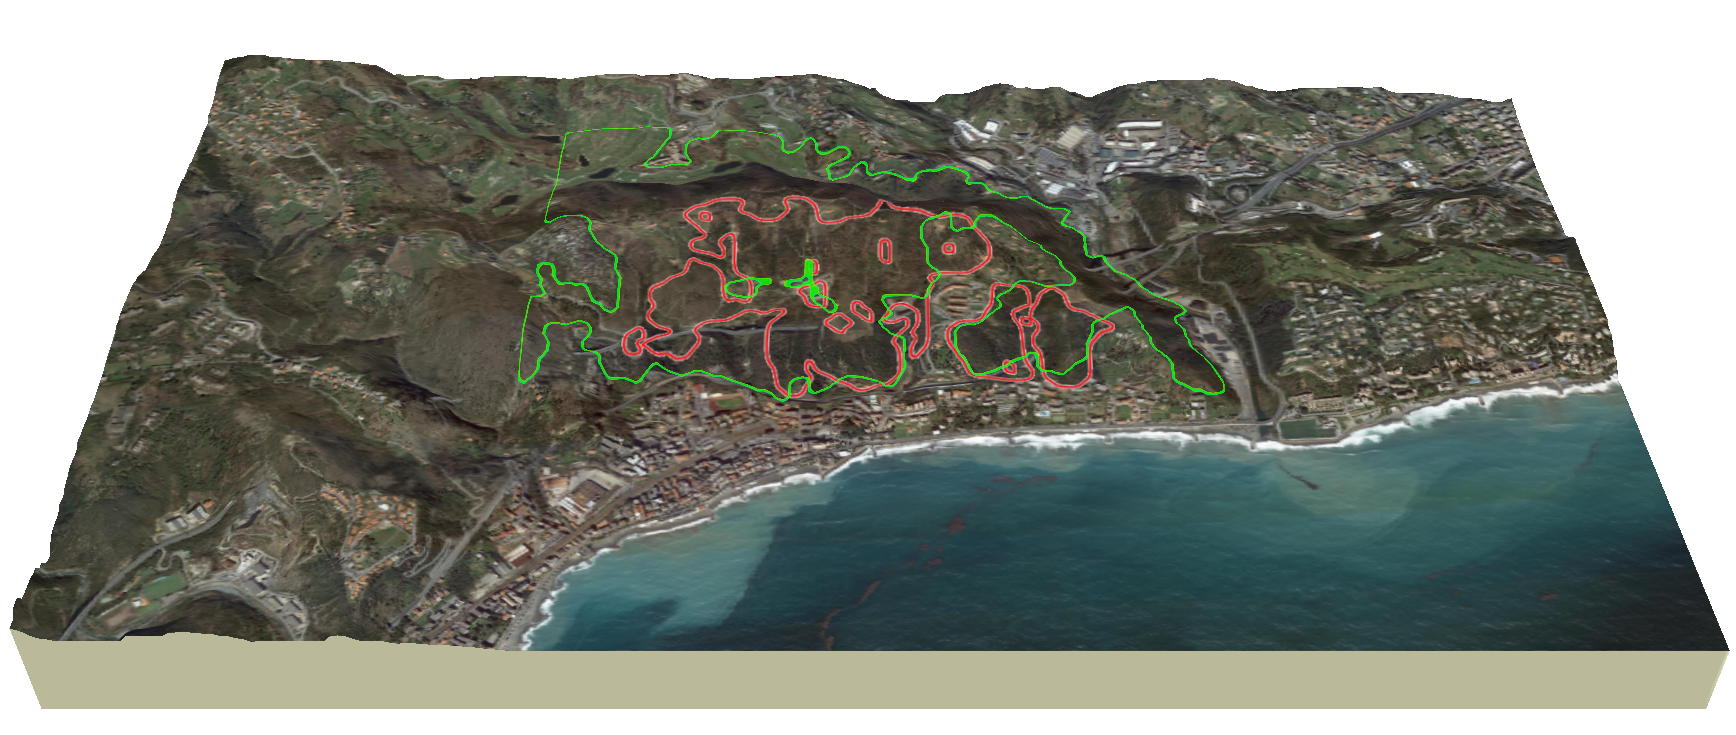
\includegraphics[width=\textwidth]{figures/cogoleto_fire_2019_ls4_1000.png}
\caption{Satellite photograph of the region where the Cogoleto Fire occurred. The area outlined in red is the extent of the actual fire; green is the simulation.}
\label{Cogoleto_satellite}
\end{figure}

Shown in Fig.~\ref{Cogoleto_satellite} are the results of a level set simulation of the fire superimposed on a satellite photograph of the area and the outline of the extent of the actual fire.

The computational domain is assembled using the open-source GIS (Geographic Information System) program called QGIS~\cite{QGIS}, extended by the qgis2fds~\cite{qgis2fds} plugin. The open-source qgis2fds plugin was specifically developed in the framework of the WUIFI-21 project\footnote{WUIFI-21: {\it High fidelity computational fluid dynamics modeling of forest fires for Wildland-Urban Interface communities resilience and protection}, an Italy-US research project financed by the Italian Ministry of Foreign Affairs and International Cooperation} for facilitating the use of geographical data for forest fire simulation and smoke pollutants dispersion in FDS.

The wind speed and direction are based on a single weather station near the point of ignition. The vegetation type is provided by a database maintained at the CIMA\footnote{International Centre on Environmental Monitoring.} Research Foundation, derived from regional forest management maps. In the simulation, the single point wind data is taken as the prevailing wind, and the local wind field is obtained via a CFD computation. The fire is simulated based on the position of the level set front; that is, when the front arrives at a given location, a fire is ignited and burns for a duration of time consistent with the specified fuel loading of that particular point on the map. 

The extent of the simulated fire, shown in green in Fig.~\ref{Cogoleto_satellite}, is greater than the actual fire, shown in red. This is not surprising given that the simulation does not include fire suppression and the rate of spread of the level set front is determined empirically for vegetation that may not exactly resemble that of this particular region.

The simulation results were compared with those obtained from CIMA Propagator~\cite{Trucchia:2020}, an experimental propagation model that has provided several European civil protection organizations with real-time fire predictions since 2009. The model has been implemented by the CIMA Foundation, its propagation model is based on stochastic cellular automata.


\section{Summary} \label{sec:summary}

The numerical methods described in this paper span the range of length scales from tens of centimeters to tens of kilometers. Obviously, these techniques support differing descriptions of the underlying fire physics, but all can be embedded within the same code base. This allows researchers to combine the different techniques in ways that were not possible when separate codes were maintained by separate organizations. With FDS, one can simulate 24 hours of fire spread in minutes of computation time using the level set function and a wind field that varies only temporally, not spatially, with no fire-atmospheric coupling. At the same time, using the same set of input parameters, one can simulate the fire at far greater resolution with much greater physical fidelity, albeit for shorter time periods and spatial extent.





\reftitle{References}


\externalbibliography{yes}
\bibliography{Vanella_Article_Atmosphere_2020,LOFM_Workshop_References}


% The following MDPI journals use author-date citation: Arts, Econometrics, Economies, Genealogy, Humanities, IJFS, JRFM, Laws, Religions, Risks, Social Sciences. For those journals, please follow the formatting guidelines on http://www.mdpi.com/authors/references
% To cite two works by the same author: \citeauthor{ref-journal-1a} (\citeyear{ref-journal-1a}, \citeyear{ref-journal-1b}). This produces: Whittaker (1967, 1975)
% To cite two works by the same author with specific pages: \citeauthor{ref-journal-3a} (\citeyear{ref-journal-3a}, p. 328; \citeyear{ref-journal-3b}, p.475). This produces: Wong (1999, p. 328; 2000, p. 475)




%% for journal Sci
%\reviewreports{\\
%Reviewer 1 comments and authors’ response\\
%Reviewer 2 comments and authors’ response\\
%Reviewer 3 comments and authors’ response
%}

%%%%%%%%%%%%%%%%%%%%%%%%%%%%%%%%%%%%%%%%%%
\end{document}

